\subsection{Perbaikan Algoritma CART}

Kesalahan yang dilakukan pada implementasi sebelumnya yaitu pada penggunaan
atribut untuk pemisahan \textit{tree}.
Jika sebuah atribut telah digunakan sebagai pemisah, dan menjadi sebuah
\textit{node} pada pohon keputusan, maka atribut tersebut tidak boleh diproses
atau menjadi pemisah kembali pada anak-anaknya, namun bisa diproses kembali
pada \textit{grandchild}-nya.

Hal seperti ini tidak pernah disebutkan dalam teks algoritma CART,
sehingga saya cukup kesulitan menemukan kesalahan yang dilakukan.

\subsection{Implementasi Random Forest}

Implemetansi algoritma \textit{ensemble} \textit{Random Forest} (RF) secara
umum mengacu pada buku Friedman, dkk. \cite{friedman2001elements}, dengan
tambahan dari video kuliah dan tulisan lain di internet.

Algoritma RF yang diimplementasikan menggunakan teknik \textit{bagging},
\textit{out-of-bag} (OOB), dan CART sebagai pengklasifikasi di setiap pohon
keputusan.

\clearpage

Berikut algoritma RF yang digunakan,

\begin{lstlisting}
FUNGSI RandomForest
INPUT
	D: dataset
	NTREE: jumlah tree
	NFEATURE: jumlah fitur yang dipilih secara acak
	NBAGGING: jumlah sub-sampel yang dipilih secara acak dengan
	replacement, dalam nilai persentase.
OUTPUT
	FOREST: kumpulan tree
VAR
	SUMOOBERROR: total galat untuk OOB
BEGIN
	SUMOOBERROR := 0.0

	FOR i = 0; i < NTREE; i++
	BEGIN
		subsample, oob := RandomPickRows(D, NBAGGING)

		subfeature := RandomPickColumns(subsample, NFEATURE)

		cartTree := CreateTree(subfeature)

		ooberror := cartTree.CountOOBError(oob)

		SUMOOBERROR += ooberror

		FOREST.AddTree(cartTree)
	END

	FOREST.AverageOOBError = SUMOOBERROR / NTREE
END
\end{lstlisting}

Hasil implementasi kemudian diuji dengan dataset \textit{Glass Identification}
\cite{evett1987rule}, dengan jumlah sample yaitu 124, jumlah fitur 9, jumlah
kelas yaitu 7 (contoh data bisa dilihat pada lampiran
\ref{appendix:dataset_glass}),
Hasilnya dalam bentuk grafik penghitungan laju galat OOB yang dapat dilihat
pada gambar \ref{fig:rf_glass}.

\begin{figure}[t]
	\centering
	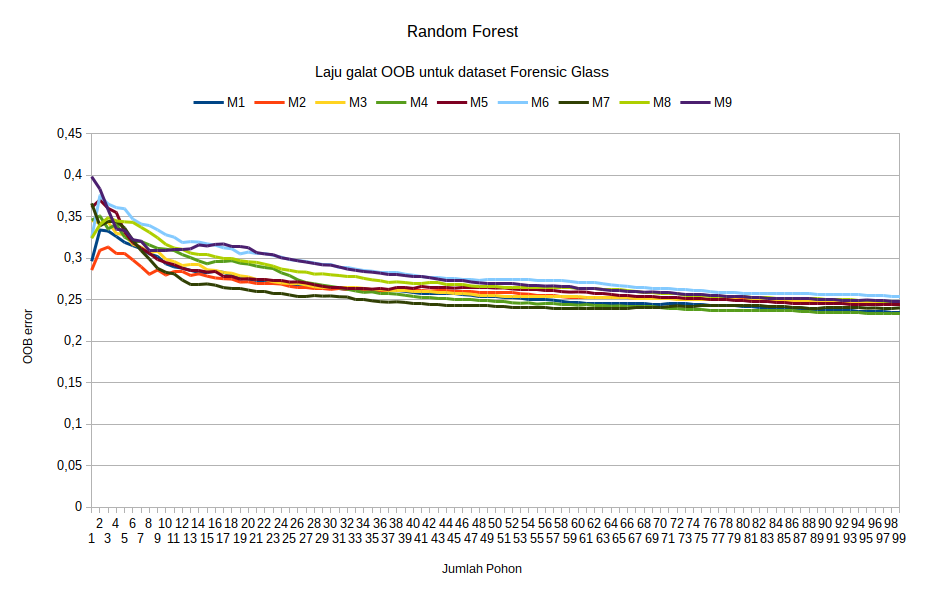
\includegraphics[keepaspectratio=true,scale=0.5]{rf_glass}
	\caption{OOB laju error pada Random Forest untuk dataset Forensic Glass
	dengan jumlah fitur secara acak dari 2 sampai 9.}
	\label{fig:rf_glass}
\end{figure}

Dataset diuji dengan mengambil dua per tiga (66\%) dari data asli untuk
\textit{bootstrap} dan sisanya digunakan sebagai latihan (OOB) untuk
mendapatkan galat, dengan jumlah tree yang digunakan yaitu 50.
